\afterpage{\null\newpage}
\chapter{Aplication of adaptive sampling\label{ch:chapter5}}

The development of an effective, scalable software platform in Chapter 5 allows us to execute adaptive sampling for larger application and larger proteins.
In this chapter adaptive sampling will be used to determine the folding and the conformational dynamics of 4 proteins. These results allows us to compare the effeciency and accuracy of adaptive sampling compared with plain molecular dynamics.  These 4 proteins range from 10 residues to 72 residues. The computational resources available limited the application to these small, fast folding proteins. 

The material in this chapter was first published in following paper: 
\\*
\cite{Extasy2019} \textbf{Hruska, E.}; Balasubramanian, V.; Ossyra, J. R.; Jha, S.; Clementi, C.; Extensible
and scalable adaptive sampling on supercomputers. arXiv (2019). URL: https://arxiv.org/abs/1907.06954.


\section{\label{sec:intro5} Introduction}
  
In Chapter 4 the efficiency and reliability of adaptive sampling strategies was compared in a statistically significant approach.  In that chapter Markov Chain trajectories were utilized to approximate the behavior of molecular dynamics trajectories. Since Markov Chain trajectories can be generated much faster than molecular dynamics trajectories a statistically significant reesults could be achieved. The limitation of this approach is that Markov Chain trajectories are only approximations and full molecular dynamics trajectories are necessary to confirm the performance of adaptive sampling.

From Chapter 4 we expect a higher speed up with adaptive sampling\cite{Adstrategies2018}.

\RED{continue}

reference data

  The results show that some adaptive sampling strategies are
both reliable, accurate and reach speed ups of one or more orders of magnitude
compared t} plain MD. For a larger, more complex protein a higher speed up is expected .


Determining the efficiency, accuracy, and reliability of a particular adaptive
sampling strategy is challenging for several reasons. Different proteins can
behave differently for different adaptive sampling strategies but limited
computational resources don't allow to adaptively sample a statistically
significant number of proteins with different strategies for comparison.
Accurate results are known only for a limited number of proteins. Despite
these challenges some performance analyzes of adaptive sampling strategies
have been performed
\cite{preto2014fast,weber2011characterization,bowman2010enhanced,Fabritiis-2014,
Adstrategies2018}. 

\subsection{\label{sec:Reference} Reference Data}

\begin{table}[H]
\centering
\caption{Adaptively sampled proteins in this study}
\label{tab:dataset-summary}
%\begin{tabular}{ccccc}
\resizebox{\columnwidth}{!}{
\begin{tabular}{|c|c|c|c|c|c|}
\hline
Protein & PDB ID & \# Residues & Folding Time ($\mu$s) \cite{lindorff2011} & Unfolding Time ($\mu$s)\\ 
\hline
Chignolin    & 5AWL                       & 10                 & 0.6                &2.2            \\
Villin       & 2F4K                       & 35                 & 2.8                &0.9            \\
BBA          & 1FME                       & 28                 & 18                 &5              \\
A3D          & 2A3D                       & 73                 & 27                 &31              \\
\hline            
\end{tabular}
}
\end{table}
To show the speed up and accuracy of the adaptive sampling method we \GRE{projected
the results of the \GRE{4} small proteins on to preexisting long MD simulations}, obtained
on the Anton supercomputer \cite{lindorff2011}. These proteins and the
reference data were investigated before \cite{reanalyze1, reanalyze2},
allowing us to demonstrate here the usefulness and reliability of the ExTASY
workflow. The \GRE{4} proteins are summarized in Table \ref{tab:dataset-summary},
their size is \GRE{from 10 to 73 residues and have a short folding time below 40 $\mu$s}.
These proteins were chosen due to their folding time which is long enough to
show the advantages of adaptive sampling with ExTASY framework, but still
reachable with our computational resources. Only the C-alpha coordinates are
used when comparing the reference data trajectories with the results from the
ExTASY framework in this work. \GRE{Since parallelization strongly affects the time to fold, we compare the results of adaptive sampling with the results of plain MD with the same number of parallel simulations, starting from the same starting configuration. Bot adaptive sampling and plain MD were executed with the ExTASY platform.}


\subsection{\label{sec:MD} Molecular dynamics simulation}

\begin{figure}[H]
   \begin{subfigure}[b]{0.6\linewidth}
   {\scalebarimg{figures2/plot_reana_61_extasy_vamp_chignolin3-free-energy-TICA2-overlap_mod.pdf}{0.98}{A)}{0mm}{-2mm}}
   \end{subfigure}%
   
   \begin{subfigure}[b]{0.6\linewidth}
   {\scalebarimg{figures2/plot_reana_61_extasy_vamp_villin3-free-energy-TICA2-overlap_mod.pdf}{0.98}{B)}{0mm}{-2mm}}
   \end{subfigure}%

  %%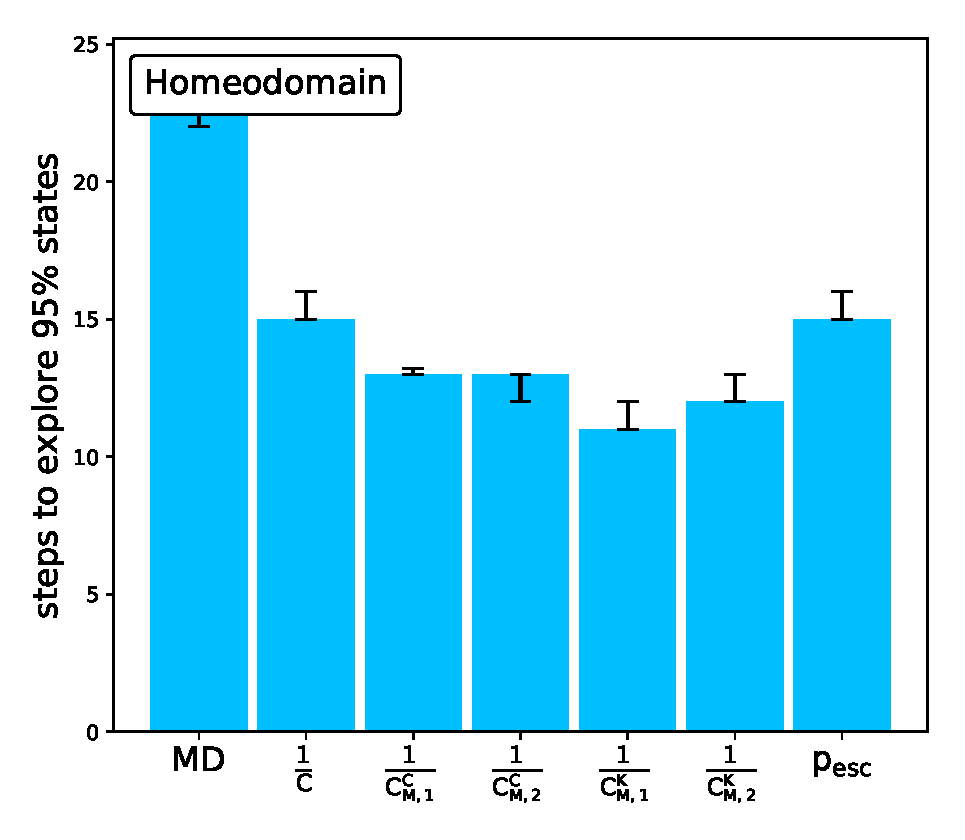
\includegraphics[width=\linewidth]{figures/UVF_7_steps10000_nparallel100_explore.eps}
  \caption{Exploration of the protein energy landscape in TICA coordinates. The
 color background shows the explored Free Energy landscape by the reference
 dataset. The black diagonal lines on top show the explored conformations by the adaptive
 sampling in this paper. The almost perfect overlap shows that the whole
 conformational landscape of \GRE{all 4 proteins was fully explored. The labels show} the location of the folded state. Individual proteins: A) Chignolin B) Villin }
\end{figure}

\begin{figure}[H]\ContinuedFloat

   
   \begin{subfigure}[b]{0.6\linewidth}
   {\scalebarimg{figures2/plot_reana_61_extasy_vamp_bba3-cmicro-free-energy-TICA2-overlap_mod.pdf}{0.98}{C)}{0mm}{-2mm}}
   \end{subfigure}%
  
   \begin{subfigure}[b]{0.6\linewidth}
   {\scalebarimg{figures2/plot_reana_61_extasy_a3d9-free-energy-TICA2-overlap_mod.pdf}{0.98}{D)}{0mm}{-2mm}}
   \end{subfigure}%

  %%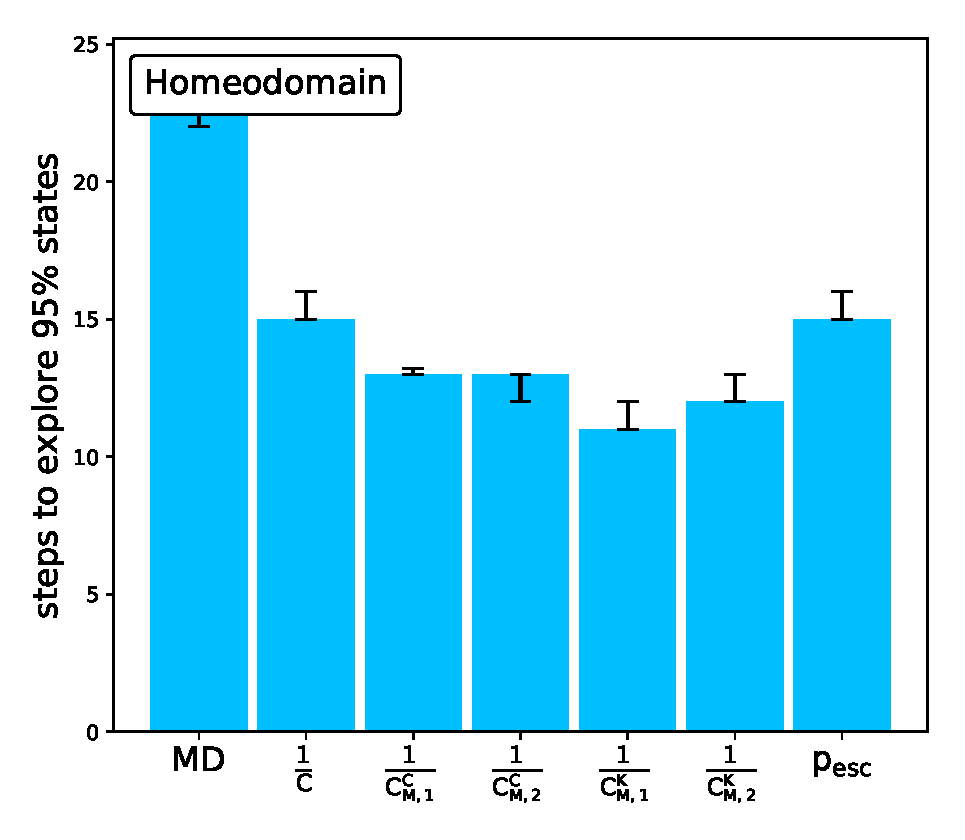
\includegraphics[width=\linewidth]{figures/UVF_7_steps10000_nparallel100_explore.eps}
  \caption{\GRE{(cont.)} Individual proteins: C) BBA D) A3D} 
  \label{fig:overlap}
\end{figure}

The MD simulations in this work were performed with \GRE{OpenMM 7.5} \cite{openMM}
using \GRE{CUDA 9.1 on the Summit supercomputer}. To reproduce the same setup
as in \cite{lindorff2011} we used CHARMM22* force field \cite{Charmm22star}
and the modified TIP3P water. The stepsize used was 5fs \GRE{or 2fs in case of protein A3D}, and the trajectories
were strided to \GRE{ to reduce the data volume}. Differently
from \cite{lindorff2011}, we used the Particle Mesh Ewald method for
long-range electrostatics due to OpenMM \GRE{settings}. For each protein, the start \GRE{configuration
is one frame in the reference dataset selected randomly from the 20\%
of frames with the highest Root Mean Square Deviation (RMSD) from the
protein crystal structure.} A short energy equilibration (1-2ns) was then
performed in the NPT ensemble to create initial coordinates for the workflows.
No further a priori information was given to the ExTASY framework except the
unfolded start conformations.

In each iteration, 50 OpenMM trajectories were simulated on 50 \GRE{GPUs on Summit with one GPU per trajectory. The length of each trajectory was 50ns
for Chignolin and Villin, 10ns for BBA and 40 ns for A3D. ExTASY scales up to
1000s of GPUs, so it} can be used to simulate even larger proteins or \GRE{a larger number of parallel walkers}.  Steps 2 and 4 were performed on \GRE{one GPU on Summit utilizing the same job as the MD simulations.}  After all the simulations are finished, the folding times, speed up and the accuracy of protein dynamics was determined by
comparing with the Anton MD simulations starting from the selected start
conformation. 
\GRE{In this paper, we illustrate the abilities of adaptive sampling and the ExTASY framework by comparing the results of adaptive sampling and plain MD for the 4 proteins. The expected variation of the time to fold for both adaptive sampling and plain molecular dynamics can reach 50\% \cite{Adstrategies2018}, caused by stochasticity. A significant increase of computational resources would be required to make the comparison between adaptive sampling and plain MD statistically significant.}


\begin{figure}[H]
   \begin{subfigure}[b]{0.6\linewidth}
   {\scalebarimg{figures2/plot_chigsummary14_pop_fraction2_2_mod3.pdf}{0.95}{A)}{0mm}{-5mm}}
   \end{subfigure}%
   
   \begin{subfigure}[b]{0.6\linewidth}
   {\scalebarimg{figures2/plot_vilsummary14_pop_fraction2_2_mod3.pdf}{0.95}{B)}{0mm}{-5mm}}
   \end{subfigure}%


  \caption{The population of explored states evolving with absolute simulation time.  Around one
  order of magnitude shorter time to solution can be reached with adaptive
  sampling compared to plain MD simulations. \GRE{For Chignolin and A3D the $cmacro$ adaptive sampling strategy was used, for Villin and BBA the $cmicro$ adaptive sampling strategy was used. Both adaptive sampling strategies are described in Section~\ref{sec:restart-strategies}. The vertical lines indicate folding events.} Individual proteins: A) Chignolin B) Villin }
\end{figure}

\begin{figure}[H]\ContinuedFloat
   \begin{subfigure}[b]{0.6\linewidth}
   {\scalebarimg{figures2/plot_bbasummary14_pop_fraction2_2_mod3.pdf}{0.95}{C)}{0mm}{-5mm}}
    \end{subfigure}%

   \begin{subfigure}[b]{0.6\linewidth}
   {\scalebarimg{figures2/plot_a3dsummary15_pop_fraction2_2_mod3.pdf}{0.95}{D)}{0mm}{-5mm}}
    \end{subfigure}%
  \caption{
  \GRE{(cont.) Proteins C) BBA D) A3D } \GRE{The plain molecular dynamics simulation of A3D has not folded despite simulating about 7 times longer than necessary for folding with adaptive sampling. Additional computational resources would allow to fold protein A3D with plain molecular dynamics too.}}
  \label{fig:Pop_explored}
\end{figure}
\section{\label{sec:results}Results and Discussion}

To analyze the efficiency of adaptive sampling, we considered several
measures. To show the completeness of the exploration, we measured the fraction
of the explored population and considered the overlap of the explored areas with the
reference dataset. This also allows us to estimate the speed up time to solution
compared to the reference method. To analyze the accuracy of the simulated
protein dynamics we compare the relative entropy of the MSM transition
matrices, and the Mean First Passage Time (MFPT) to the folded state, as
detailed below.

\subsection{\label{sec:time-fold}Comparison of Exploration}
\begin{figure}[H]
   
   \begin{subfigure}[b]{0.7\linewidth}
   {\scalebarimg{figures2/plot_vilsummary14_rel_ent_fold_4_mod2.pdf}{1}{}{0mm}{-3mm}}
   \end{subfigure}%
   
  \caption{
  Relative entropy between the MSM transition matrices generated during the
  ExTASY exploration and from the \GRE{plain MD comparison run}. Results \GRE{for protein Villin}. The relative entropy decreases with increasing number of adaptive
  sampling iterations. }
  \label{fig:rel_ent}
\end{figure}

The whole explored energy landscape of the protein cannot be visualized due to
the high dimensionality of the raw trajectories, but the explored landscape in
the reduced TICA coordinates is shown in
Figure~\ref{fig:overlap}. The colored background shows the explored free energy landscape of
the reference dataset and the shaded foreground shows the region of this landscape explored
by the adaptive sampling. The whole energy landscapes of the proteins\GRE{ Chignolin, Villin, BBA and A3D were} explored by ExTASY. The small differences in overlap could be
caused by the differences in the long-range electrostatics setup and stochastic \GRE{nature of the exploration}. The case of protein A3D shows that for larger protein the computational resources to fully explore the energy landscape rise significantly. \GRE{Our computational resources allowed us to fold A3D with adaptive sampling, but not with plain molecular dynamics. The plain molecular dynamics simulation didn't fold even when simulating about 7 times longer than the time to fold with adaptive sampling. To show that adaptive sampling works with different adaptive sampling strategies, we folded Chignolin and A3D with the $cmacro$ adaptive sampling strategy and  the $cmicro$ adaptive sampling strategy was used to fold Villin and BBA.}

To show how effectively the whole protein landscape is explored, we
use the fraction of the total population explored as a function of time.
Here we select all the states which are explored at a certain time and
compare with all possible states (as obtained from the reference simulations).
To represent the different importance of different states we weight the
explored states with their stationary weight. The population of each microstate
is calculated as the stationary weight of that microstate from the MSM analysis of
the reference dataset. Figure~\ref{fig:Pop_explored} reports the comparison of
the explored populations as a function of time for the reference dataset and
the ExTASY results. \GRE{For all 4 proteins, adaptive sampling explores the protein energy landscape slightly faster and folds significantly faster. The folding speed up of adaptive sampling compared to plain MD is 170\% for Chignolin, 20\% for Villin, 380\% for BBA, and more than 690\% for A3D. The larger speed up for A3D is in line with the prediction that for larger and more complex protein adaptive sampling achieves a larger speed up\cite{Adstrategies2018}. The exact speed up for the protein A3D could not be determined due to limited computational resources. The quantitative comparison between adaptive sampling and plain MD is not statistically significant due to the low sample size caused by limited computational resources.}

The x-axis in Figures~\ref{fig:Pop_explored}-\ref{fig:mfpt}
is absolute simulation time to show the improvement of time to solution with ExTASY.
Absolute simulation time is the length of one trajectory in Step 1 times the number of iterations.
When all the trajectories in Step 1 are run in parallel, the absolute simulation time
shows the time to solution independent of the used hardware. The effects of parallelization
on the time to solution for adaptive sampling were explored in \cite{Adstrategies2018},
generally \GRE{parallelization} decreases the time to solution.

\begin{figure}[H]
   \begin{subfigure}[b]{0.5\linewidth}
   {\scalebarimg{figures2/plot_chigsummary14_mfpt_unfold_3_mod2.pdf}{1}{A)}{0mm}{-2mm}}
   \end{subfigure}%
   
   \begin{subfigure}[b]{0.5\linewidth}
   {\scalebarimg{figures2/plot_vilsummary14_mfpt_unfold_3_mod2.pdf}{1}{B)}{0mm}{-2mm}}
   \end{subfigure}%
   
   \begin{subfigure}[b]{0.5\linewidth}
   {\scalebarimg{figures2/plot_bbasummary14_mfpt_unfold_3_mod2.pdf}{1}{C)}{0mm}{-2mm}}
    \end{subfigure}%
  \caption{
  MFPT from \GRE{folded to unfolded states evolving as
  more data is available after more adaptive sampling iterations. The red line is adaptive sampling, the blue line is plain MD with the same parallelization as adaptive sampling. The black dashed line shows the reference values for Anton simulation trajectories\cite{lindorff2011}.}   
  Individual proteins: A) Chignolin B) Villin C) BBA } 
  \label{fig:mfpt}
\end{figure}

\subsection{\label{sec:kinetics}Comparison of Protein Dynamics}


To track the convergence of protein dynamics in the adaptive sampling workflow,
one can use the relative entropy \cite{bowman2010enhanced} between the
MSM transition matrix of the reference data, $P_{ij}$, and the MSM transition matrix
of the analyzed data, $Q_{ij}$.
A relative entropy can be calculated between each microstate in the analyzed
and the reference transition probabilities from this state. By averaging the
relative entropy for each state weighted by the stationary probability over all
microstates we obtain the relative entropy between the two transition matrices.
The relative entropy
$D(P||Q)$ is then given by
\begin{equation}
D(P||Q)=\sum_{i,j}^{N}s_{i}P_{ij}\ln\frac{P_{ij}}{Q_{ij}}. 
\end{equation}
where $s_{i}$ is the equilibrium probability of state $i$. The transition
matrices $P_{ij}$ and $Q_{ij}$ have to use exactly the same dimension reduction
and same clustering.
As zero counts in the transition matrices can cause divergence of the relative
entropy, a pseudo-count of $1/N$ (where $N$ is the length of the simulation) is
added to each element of the count matrices
before normalizing the rows to get the transition matrices
\cite{bowman2010enhanced}. \GRE{ The relative entropy for a certain simulation time is
obtained from all the trajectories up to the specified simulation time. By definition, the relative entropy of the full reference
trajectory is zero.  Figure~\ref{fig:rel_ent} shows how the relative
entropy decreases with increasing simulation time for both the adaptive sampling and plain MD simulations. The adaptive sampling strategy decreases the relative entropy faster at the beginning, later in the simulation plain MD decreases the relative entropy faster. While the sample size is small, this confirms that the chosen investigated sampling strategy is effective at exploring the protein landscape, but not optimized in the later steps of converging protein kinetics \cite{Adstrategies2018}. Different adaptive sampling strategies which are optimized for converging the kinetics could improve the behavior of adaptive sampling towards the end of the simulation.}

\GRE{An additional measure to compare the convergence of the kinetic behavior of the proteins is Mean First Passage Time (MFPT). MFPT measures the mean time to reach for the first time another state from one state. Here the two states are the folded and unfolded states, both defined as an ensemble of MSM states based on the TICA coordinates. The folded and unfolded MSM states for the proteins were
defined by their TICA positions. Figure~\ref{fig:mfpt} shows how the MFPT from the
folded to the unfolded state converges as a function of simulation time, for both the adaptive sampling and the plain MD simulations. The reference MFPT obtained from Anton trajectories shows that the results of both plain MD and adaptive sampling can be about one order magnitude off the reference value. Adaptive sampling shows larger errors in the case of Chignolin and Villin, but a smaller error in the case of BBA compared to plain MD. The small sample size prevents us to conclude if plain MD or adaptive sampling converges faster. Additionally, the used adaptive sampling strategies are not optimized or validated for convergence of kinetics. The slow convergence of MFPT for Chignolin and Villin shows that accurate kinetic values require a long sampling and that kinetic values from both plain MD and adaptive sampling have relatively large uncertainties. The sizes of the MFPT errors are similar to what was obtained with the HTMD framework \cite{doerr2016htmd}. For protein A3D the convergence of MFPT could not be compared since the plain MD simulation did not fold. Additional investigation in the theory of convergence of kinetic values for protein sampling methods would allow understanding these results better.}  


\section{\label{sec:conclusion}Conclusion}

We have shown that the ExTASY framework \cite{Extasy2016} can effectively
perform adaptive sampling, as exemplified \GRE{by adaptively sampling 4 proteins using deep learning. The free energy landscape of the 4 proteins was fully sampled. In comparison to a plain molecular dynamics simulation with the same parallelization a small but not statistically significant speed up in the range of 20\% to 690\% could be observed. These speed ups are in line with predictions \cite{Adstrategies2018} which rise with the size of the proteins. The MFPT times converged for both adaptive sampling and plain MD to values similar to the reference values. For protein BBA the adaptive sampling converges the MFPT significantly faster than plain MD, but proteins Chignolin and Villin show as slower convergence. The expected large stochastic fluctuation expected in both plain MD and adaptive sampling prevents a statistically significant comparison of MFPT times between plain MD and adaptive sampling. The sample size in this paper was limited by computational resources. Additional adaptive sampling strategies optimized in recovering the kinetics would improve the results of adaptive sampling for MFPT convergence. The relative entropy between the transition matrix of the MSM computed during the adaptive
sampling and the MSM of the plain MD decreases steadily with the
simulation time, the adaptive sampling converges here faster than plain MD at the beginning of the simulation. The differences in speed of convergence are caused by the choice of adaptive sampling strategy, which are validated for the exploration of protein energy landscapes, but not optimized to reach accurate protein kinetics. Due to the stochasticity, the comparison of the speed up between adaptive sampling and plain MD is not statistically significant. For statistically significant results a significant increase in computational resources would be required.}
\GRE{The modularity of the ExTASY framework reduces the time spent by domain experts in executing
adaptive sampling in a scalable fashion on diverse platforms. Scalability of over 1000 GPUs and 1000 simultaneous protein replicas was demonstrated on Summit. This scalability doesn't come at the cost of inflexibility, due to the design and implementation of the ExTASY framework \cite{Extasy2016}, ExTASY can be
easily modified for different proteins or MD
simulation software. ExTASY can also be easily extended to different adaptive
sampling strategies and platforms. The ExTASY framework is available open-source at} \href{https://github.com/ClementiGroup/ExTASY}{https://github.com/ClementiGroup/ExTASY}. \GRE{The flexibility of ExTASY allowed this framework to be the first open-source adaptive sampling platform which supports deep learning or asynchronous execution.}
